\chapter{Lezione 10 - Enterprise Content Management (ECM), gestione dei contenuti per l'impresa}

Parleremo dell'Enterprise Content Management, gestione dei contenuti per l'impresa.

Gli argomenti che affronteremo sono una serie di concetti di base, una e più definizioni del settore della gestione dei contenuti di base e l'evoluzione storica che ha avuto questo settore.

\FloatBarrier
\begin{figure}[H]
  \centering
  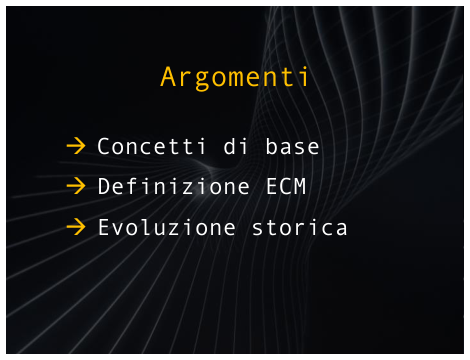
\includegraphics[width=0.50\textwidth,
                    trim=40 100 40 60, % L B R T
                    clip]
                    {images/Lez10_p01_fig_02}
  % \caption{Sommario}
  % \label{fig:Lez15_p06_fig_02}
\end{figure}
\FloatBarrier
\noindent

Vediamo i concetti di base.

\FloatBarrier
\begin{figure}[H]
  \centering
  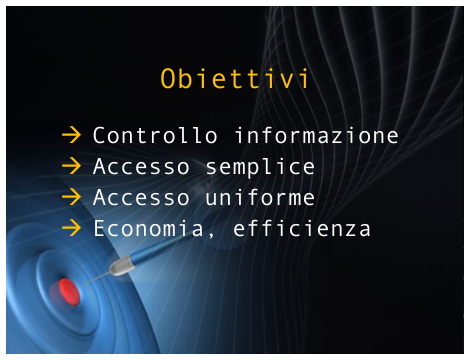
\includegraphics[width=0.50\textwidth,
                    trim=40 100 40 60, % L B R T
                    clip]
                    {images/Lez10_p01_fig_04}
  % \caption{Sommario}
  % \label{fig:Lez15_p06_fig_02}
\end{figure}
\FloatBarrier
\noindent

Gli obiettivi dell'Enterprise Content Management sono innanzitutto il controllo dell'informazione.
Per controllo dell'informazione noi intendiamo sia la ricerca, le attività che riguardano la localizzazione, la scoperta, il raccoglimento della informazione, ma anche la valutazione della qualità, dell'autorità dell'informazione, la gestione dell'eventuale  versioning.

L'accesso semplice all'informazione.
L'informazione deve essere organizzata in modo tale che possa essere raggiungibile con semplicità, velocemente e deve essere recuperata l'informazione di interesse, non ci devono essere ridondanze o informazioni inutili.

L'accesso uniforme.
L'obiettivo a cui faceva riferimento l'accesso uniforme è perché i contenuti o le informazioni trasportate dai contenuti o i documenti che contengono questi contenuti devono essere acceduti alla stessa maniera sia dai vari reparti di uno stesso dipartimento, di una stessa impresa che fanno uso degli stessi documenti, quindi accedono allo stesso sistema di gestione, sia anche chi dall'esterno ha la possibilità di accedere a questi documenti deve poter accedere in  maniera analoga per quanto riguarda l'accessibilità dell'informazione non la protezione o qual è l'insieme di informazioni a cui possono avere accesso.

Economia ed efficienza.
Gli strumenti di supporto, i metodi per l'organizzazione delle informazioni, i documenti e i contenuti devono permettere sia una gestione rapida, efficiente nel senso che le informazioni devono essere recuperate in tempo rapido e in maniera soddisfacente, in maniera esaustiva e in maniera economica.
Quindi sia in termini di tempo sia anche l'informazione organizzata deve permettere dei risparmi rispetto a ricerche lunghe, laboriose, non si sa in quale archivio verranno recuperate.

\FloatBarrier
\begin{figure}[H]
  \centering
  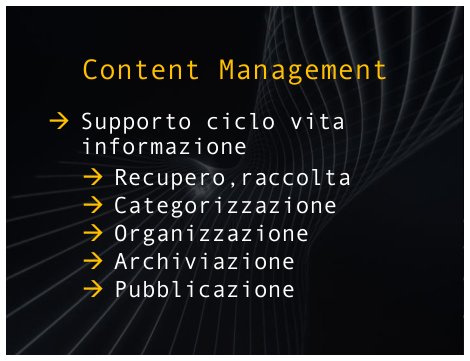
\includegraphics[width=0.50\textwidth,
                    trim=40 80 40 40, % L B R T
                    clip]
                    {images/Lez10_p01_fig_05}
  % \caption{Sommario}
  % \label{fig:Lez15_p06_fig_02}
\end{figure}
\FloatBarrier
\noindent

Il content management è l'insieme di attività a supporto del ciclo di vita della informazione.
A partire dal recupero, la raccolta di queste informazioni che possono essere raccolte già organizzate o recuperate da altre archivi, recuperate per esempio in internet, recuperate da pubblicazioni, recuperate da bollettini o da messaggi che ci vengono inviati da collaboratori, oppure digitalizzate, acquisite da apparecchiature di laboratorio, acquisite da device mobili che trasportano gli utenti e così via.

L'informazione una volta raccolta, una volta acquisita, deve però essere categorizzata.

Categorizzata significa che devono essere organizzati in temi, in gruppi specifici per uno stesso argomento.

Organizzate perché possano essere utilmente archiviate e raggiungibili con semplicità o a seguito di percorsi di navigazione o con accesso diretto, quindi formulando dell'interrogazione a sistemi per la gestione di base di dati se questi contenuti sono organizzati come dati formattati o con sistemi di information retrieval o nel caso che stiamo vedendo ora sistemi di content management, anche sistemi general purpose più estesi, più rivolti a una varietà di tipi di supporto per i contenuti possibile.

Le informazioni sono quindi archiviate per una loro successiva pubblicazione.
Vedremo come l'attività di pubblicazione comprende da una parte la scelta delle informazioni che possono essere pubblicate, quindi la valutazione della loro riservatezza, dall'altra parte una scelta di porre magari temporaneamente delle informazioni, dei contenuti pubblici e successivamente toglierli dall'accesso a tutte le persone.

La pubblicazione di informazioni richiede anche un'attenzione, come vedremo, alla loro presentazione, al modo in cui le informazioni possono o devono essere presentate anche a causa dei canali attraverso cui sono trasportati o attraverso cui sono presentate.

\FloatBarrier
\begin{figure}[H]
  \centering
  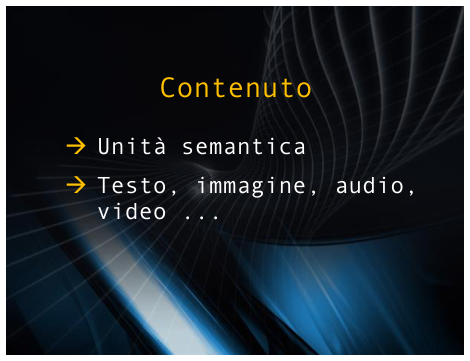
\includegraphics[width=0.50\textwidth,
                    trim=40 80 40 40, % L B R T
                    clip]
                    {images/Lez10_p01_fig_06}
  % \caption{Sommario}
  % \label{fig:Lez15_p06_fig_02}
\end{figure}
\FloatBarrier
\noindent

Ma cos'è un contenuto?
Perché parliamo di content management e non di information o document management?

Il contenuto fa riferimento a un'unità semantica, il contenuto fa riferimento a un significato o a un senso che ci interessa.

Il contenuto, questa unità semantica, può essere rappresentata da un testo, da un'immagine, da un audio o da un video.
Allora abbiamo un'unità semantica che può essere mostrata come racconto, come testo, oppure rappresentata da una foto o da un'immagine artificiale di laboratorio, può essere un audio, una registrazione o un filmato.
I formati con cui le informazioni che costituiscono il contenuto sono organizzate, sono formattate, non è rilevante.
Noi facciamo riferimento al valore semantico, al significato, al valore di senso che ha per noi quell'unità.

\FloatBarrier
\begin{figure}[H]
  \centering
  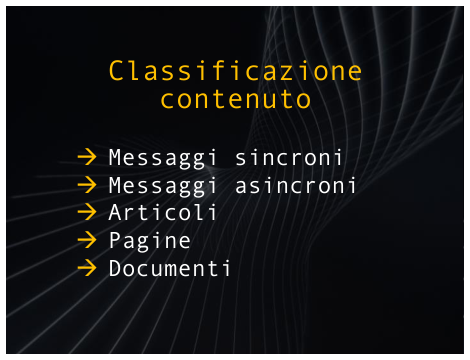
\includegraphics[width=0.50\textwidth,
                    trim=40 40 40 40, % L B R T
                    clip]
                    {images/Lez10_p02_fig_01}
  % \caption{Sommario}
  % \label{fig:Lez15_p06_fig_02}
\end{figure}
\FloatBarrier
\noindent

Il contenuto viene tipicamente classificato sulla base del supporto, sulla base della forma che ha l'informazione, il messaggio che lo trasporta.
Quindi avremo messaggi sincroni, per esempio i messaggi delle chat, i messaggi nella messageria istantanea, oppure possono essere classificati in messaggi asincroni come nel caso delle mail o dei forum, quando il messaggio può essere letto nel momento preferito dal ricevente.

La categoria dei messaggi sincroni fanno anche parte gli sms che adesso sono uno strumento di comunicazione molto diffuso.

Gli articoli come ad esempio vedremo delle pagine wiki piuttosto che gli interventi, i post in un blog, gli interventi in una discussione gestita attraverso un blog, pagine web o pagine di un sistema wiki o documenti, documenti formattati come articoli tradizionali con una struttura a indice, una paragraffatura e delle caratteristiche che adesso andiamo a vedere.

\FloatBarrier
\begin{figure}[H]
  \centering
  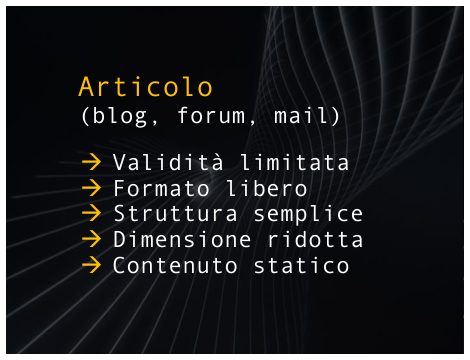
\includegraphics[width=0.50\textwidth,
                    trim=40 60 40 60, % L B R T
                    clip]
                    {images/Lez10_p02_fig_02}
  % \caption{Sommario}
  % \label{fig:Lez15_p06_fig_02}
\end{figure}
\FloatBarrier
\noindent

L'articolo è trasportato tipicamente come contributo nei blog, nei forum o come mail, ha una validità piuttosto limitata nel tempo, la durata di interesse di queste informazioni è molto limitata.

E' breve e l'utente può selezionare quali messaggi archiviare per valore storico, per cronaca, per mantenere una documentazione su un'attività che ha una durata superiore.
Questo tipo di supporto, l'articolo, ha un formato libero, possono essere formattati in qualsivoglia maniera, non ha rilevanza per il tipo di contenuto che viene trasportato, perché il contenuto avrà una struttura semplice, come può essere un paragrafo, un concetto non strutturato.

La struttura del supporto dell'articolo è una struttura semplice, come una mail, può essere un testo, può essere un messaggio mandato in un post in cui esprimiamo il nostro concetto, esprimiamo il nostro problema.

La dimensione è ridotta, sono messaggi piuttosto sintetici anche perché abbandonare la sintesi significa andare verso una rappresentazione più strutturata e non un supporto del genere e quindi dovremo acquisire un modo di trasportare contenuti più strutturato, più complesso.

Il contenuto è statico, ha valore limitato e non viene modificato, sia per la semplicità del contenuto, sia anche per la validità temporale ridotta.

\FloatBarrier
\begin{figure}[H]
  \centering
  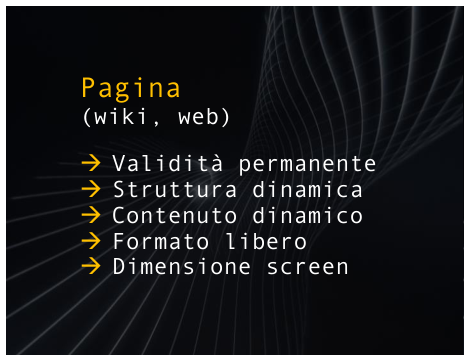
\includegraphics[width=0.50\textwidth,
                    trim=40 60 40 60, % L B R T
                    clip]
                    {images/Lez10_p02_fig_03}
  % \caption{Sommario}
  % \label{fig:Lez15_p06_fig_02}
\end{figure}
\FloatBarrier
\noindent

Il successivo tipo di supporto è la pagina.
Con validità permanente è un tipo di supporto che viene utilizzato nei sistemi wiki, quindi sistemi di creazione, di gestione dei documenti partecipati in cui più persone possono contribuire alle nuove versioni dei documenti, oppure pagine web che tipicamente hanno una validità permanente, una durata nel tempo come contenuto, stiamo parlando del contenuto che è trasportato da questa pagina, hanno una struttura dinamica a fronte di un significato di interesse e duratura nel tempo della pagina.

La pagina viene modificata, aggiornata nella grafica ma non solo nella grafica, anche nel contenuto.
Il contenuto viene aggiornato, la pagina wiki per esempio cambia quotidianamente, mantiene l'argomento, mantiene la struttura complessiva o l'interesse del contenuto, del senso che viene trasportato, ma può essere aggiornata sia nella presentazione, nella sua struttura, sia nel tipo di contenuto, le informazioni che contiene possono essere aggiornate, anche perché la durata temporale è più lunga.

Il formato è libero, non ha rilevanza in questi casi la struttura con cui viene organizzato e presentato il contenuto.
La dimensione, essendo un documento solitamente di consultazione in navigazione, è suggerito che questi supporti di contenuti abbiano la dimensione di una videata.

E noto che nella visualizzazione delle pagine web o delle strutture presentate come pagine web, o come documenti analoghi alle pagine web, sia consigliabile evitare l'uso delle barre di scorrimento, le scroll bar, fare in modo che il livello di sintesi sia tale da poter essere rappresentato in una semplice videata.
Queste sono indicazioni di massima per una ottimizzazione della realizzazione del contenuto, della pagina di presentazione.

\FloatBarrier
\begin{figure}[H]
  \centering
  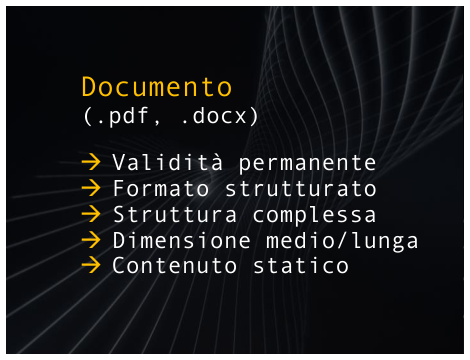
\includegraphics[width=0.50\textwidth,
                    trim=40 60 40 60, % L B R T
                    clip]
                    {images/Lez10_p02_fig_04}
  % \caption{Sommario}
  % \label{fig:Lez15_p06_fig_02}
\end{figure}
\FloatBarrier
\noindent

Il documento PDF o DocX come formato ha validità permanente.
I formati sono solo esemplificativi.
Facciamo riferimento a quei contenuti che sono strutturati, sono trasportati in un formato complesso perché il contenuto, oltre ad avere una validità permanente, ha una struttura piuttosto complessa, ha una paragraffatura, ha spesso a una struttura a priori, un titolo, degli autori o delle organizzazioni, autori di riferimento, un sommario, una paragraffatura, eventuali fonti di riferimento, la struttura che noi diamo a quelli che tradizionalmente vengono chiamati documenti, vengono utilizzati per gli articoli scientifici, per i rapporti di lavoro, ma anche per le lettere professionali, le lettere di lavoro.

Hanno un formato strutturato, perché è il senso che trasportiamo è complesso , quindi l'unità semantica è un'unità strutturata, può essere composta di più unità correlate, quindi la rappresentazione seguirà questa complessità, sarà specchio di questa complessità e il formato sarà strutturato.

La struttura anche semantica è più complessa dei supporti che abbiamo visto precedentemente, l'unità è composta di più di più parti, è un'unità per un senso complessivo, è unitaria per il completamento della trattazione dell'argomento, ma può essere scomposta in sottoparti di significato autonomo, i paragrafi.

La dimensione dei documenti è medio lunga.
Medio lunga va dall'articolo al libro, quindi può andare dalle unità di pagine fino alle centinaia di pagine, certo il limite sta nella trasportabilità, nella maneggevolezza o nella consultabilità di questo supporto che fornisca una possibilità di consultare il documento, quindi analizzare il contenuto trasportato in maniera agile e efficace.

Il contenuto dei documenti è statico.
Statico non indica tanto che è vietato l'aggiornamento, indica che sono documenti preelaborati, preelaborati vuol dire risultati di studio, risultati di analisi, sono rapporti, sono risultati di un'attività ponderata, di un'attività meditata e ci si aspetta che gli aggiornamenti possano essere meno frequenti.

Un articolo scientifico, un rapporto può essere modificato, un libro presenta le ristampe, le nuove edizioni anche nella sua versione online, ma naturalmente saranno più rare che non una pagina web che è prodotta in maniera accurata ma rapida per fornire informazioni che devono essere sulla piazza velocemente.

\FloatBarrier
\begin{figure}[H]
  \centering
  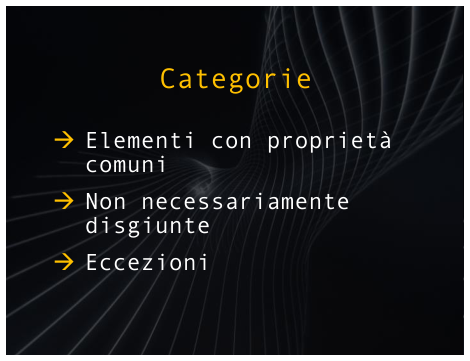
\includegraphics[width=0.50\textwidth,
                    trim=40 60 40 60, % L B R T
                    clip]
                    {images/Lez10_p02_fig_05}
  % \caption{Sommario}
  % \label{fig:Lez15_p06_fig_02}
\end{figure}
\FloatBarrier
\noindent


Le categorie sono elementi con proprietà comune.
A cosa serve la categorizzazione dei contenuti? Serve per organizzarli.

Sappiamo che nella società dell'informazione la diffusione delle informazioni è diventata estrema, tantissime informazioni sono disponibili, tantissime informazioni servono per svolgere le attività che comunemente svolgiamo, così le dobbiamo organizzare.
Le categorie sono tematiche, sono mentali, sono istintive, non sono necessariamente disgiunte, a differenza per esempio dalle classi.

La classificazione invece richiede che ogni elemento possa appartenere a una sola classe.

Le categorie diciamo servono per raggruppare, clusterizzare i contenuti per tema.

Inoltre dobbiamo considerare l'eccezione. Sono contenuti che non rispettano determinate regole comuni e possono quindi essere gestite consapevolmente al di fuori delle norme, regole comuni a cui sono sottoposti gli altri contenuti e i supporti che li trasportano.

Alla fine di questo argomento vi propongo uno spunto di riflessione.
Quali classi di contenuti utilizzate nell'attività professionale o formativa?
Inoltre dettagliate questo spunto considerando di ordinare quanto svolto in precedenza in base alla frequenza d'uso.

\section{Definizione dell'Enterprise Content Management}

\FloatBarrier
\begin{figure}[H]
  \centering
  
\includegraphics[width=0.50\textwidth,
                    trim=40 60 40 60, % L B R T
                    clip]
                    {images/Lez10_p03_fig_03}
  % \caption{Sommario}
  % \label{fig:Lez15_p06_fig_02}
\end{figure}
\FloatBarrier
\noindent

Vediamo ora la definizione dell'enterprise content management o meglio analizziamo alcune delle definizioni proposte.
L'AIIM, l'association for information and image management international, è un'organizzazione no profit per la formazione di ricerche di mercato, certificazione e definizione di standard.
Nasce nel 1943, assume questa denominazione nel 1982, ha sede negli Stati Uniti.

\FloatBarrier
\begin{figure}[H]
  \centering
  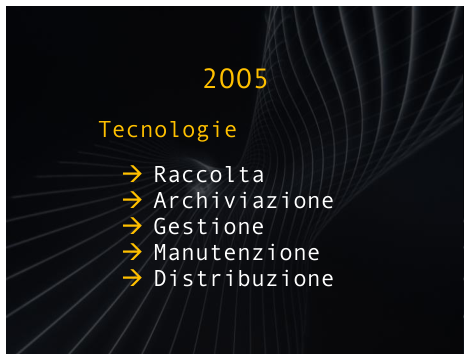
\includegraphics[width=0.50\textwidth,
                    trim=40 60 40 60, % L B R T
                    clip]
                    {images/Lez10_p03_fig_04}
  % \caption{Sommario}
  % \label{fig:Lez15_p06_fig_02}
\end{figure}
\FloatBarrier
\noindent

Nel 2000 ha dato la prima definizione di enterprise content management, definizione che è stata sviluppata, modificata e divulgata o ha trovato un'ampia divulgazione nel 2005 come insieme di tecnologie per la raccolta, l'archiviazione, la gestione, la manutenzione e la distribuzione di contenuti e documenti di lavoro.

Che differenza poniamo tra contenuti e documenti di lavoro?
I contenuti fanno riferimento al valore semantico, all'unità semantica trasportata, i documenti di lavoro fanno riferimento al tipo di supporto.

Il documento è un supporto più strutturato e valido nel tempo.

\FloatBarrier
\begin{figure}[H]
  \centering
  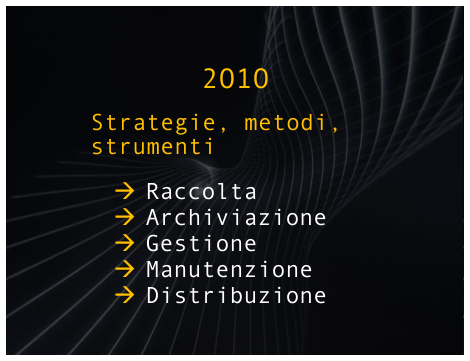
\includegraphics[width=0.50\textwidth,
                    trim=40 40 40 60, % L B R T
                    clip]
                    {images/Lez10_p03_fig_05}
  % \caption{Sommario}
  % \label{fig:Lez15_p06_fig_02}
\end{figure}
\FloatBarrier
\noindent

Nel 2010 l'insieme di tecnologie viene modificato nella definizione come insieme di strategie, metodi e strumenti per la raccolta, per l'archiviazione, per la gestione, manutenzione e distribuzione dei contenuti.

La differenza è proprio nella considerazione che se inizialmente si dava al content management una valenza tecnologica legata alle tecnologie di supporto, adesso si è riconosciuto che il settore si occupa, studia e propone sia strategie sia metodi, eventualmente supportati da strumenti tecnologici.

\FloatBarrier
\begin{figure}[H]
  \centering
  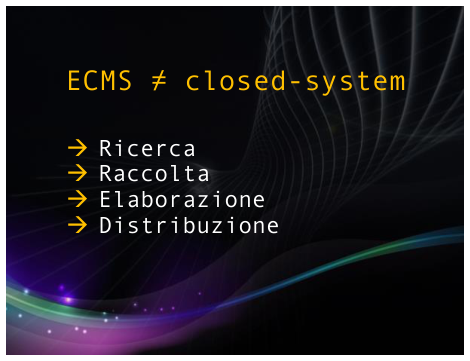
\includegraphics[width=0.50\textwidth,
                    trim=40 100 40 60, % L B R T
                    clip]
                    {images/Lez10_p03_fig_06}
  % \caption{Sommario}
  % \label{fig:Lez15_p06_fig_02}
\end{figure}
\FloatBarrier
\noindent

Assimilando queste definizioni nella pratica si evidenzia che l'enterprise content management system non è un sistema chiuso a configurazione fissa, ma fa riferimento a un termine complessivo, un termine ombrello che racchiude il supporto, la considerazione, la gestione della ricerca, della raccolta, dell'elaborazione e della distribuzione di contenuti.

\FloatBarrier
\begin{figure}[H]
  \centering
  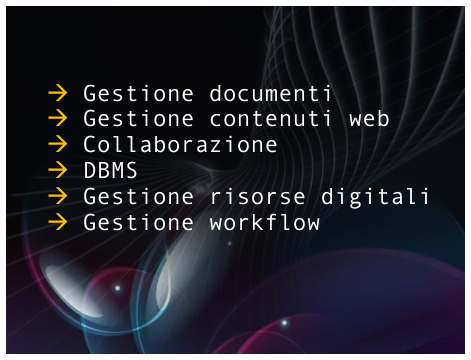
\includegraphics[width=0.50\textwidth,
                    trim=40 100 40 60, % L B R T
                    clip]
                    {images/Lez10_p04_fig_01}
  % \caption{Sommario}
  % \label{fig:Lez15_p06_fig_02}
\end{figure}
\FloatBarrier
\noindent

Nella gestione dei documenti che li trasportano eventualmente gestiti, trasmessi, prodotti online, quindi attraverso il web o attraverso i servizi offerti; la collaborazione, quindi la possibilità di produrre, utilizzare, archiviare in maniera comunitaria, in maniera comune, partecipata i contenuti o meglio i loro supporti che siano pagine piuttosto che documenti; la gestione delle basi di dati nel caso i contenuti siano trasportati anche da dati strutturati e pure la gestione di qualsiasi tipo di risorse digitali a prescindere dal fatto che siano articoli piuttosto che documenti, piuttosto che dati strutturati.

Inoltre, in questa definizione di content management è suggerita la possibilità di gestire workflow, flussi di attività, suggerimento che non sempre è soddisfatto a causa della complessità o è soddisfatto in maniera limitata a causa della complessità della gestione di una funzionalità per i workflow.

\FloatBarrier
\begin{figure}[H]
  \centering
  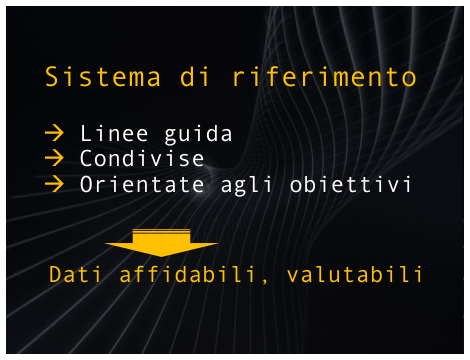
\includegraphics[width=0.50\textwidth,
                    trim=40 40 40 60, % L B R T
                    clip]
                    {images/Lez10_p04_fig_02}
  % \caption{Sommario}
  % \label{fig:Lez15_p06_fig_02}
\end{figure}
\FloatBarrier
\noindent

%26:34

Per una buona gestione dei contenuti è necessario definire un comune sistema di riferimento che sia basato su linee guida per questa gestione che siano condivise dai vari utenti, dagli autori, dagli attori di questa attività, orientate agli obiettivi comuni in modo che i dati utilizzati, i dati offerti, siano prodotti da dati affidabili e siano consultabili per la valutazione ma anche sottoponibili per la verificarne la loro provenienza.

\FloatBarrier
\begin{figure}[H]
  \centering
  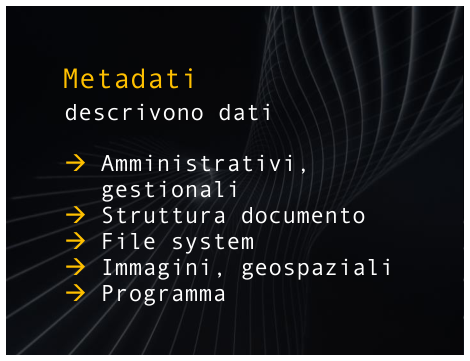
\includegraphics[width=0.50\textwidth,
                    trim=40 40 40 60, % L B R T
                    clip]
                    {images/Lez10_p04_fig_03}
  % \caption{Sommario}
  % \label{fig:Lez15_p06_fig_02}
\end{figure}
\FloatBarrier
\noindent

Per questo un elemento basilare sono i metadata, dati che descrivono dati; possono essere di diversi tipi, amministrativi gestionali, possono essere descrittivi della struttura del documento, facciamo riferimento per esempio alle pagine web che contengono una testata che descrive il loro contenuto e dà anche informazioni ai crawler che navigano per la rete, consultano gli spazi web per alimentare gli archivi dei motori di ricerca o consideriamo anche le schede catalografiche di un documento archiviato in biblioteca in cui viene proposta eventualmente l'indice, la table of contents, un sommario o una presentazione della sua struttura, titolo, autore editore.

Possono essere descrittivi del file system, nome del file, la grandezza del file, la collocazione, la data di produzione e eventualmente il peso.

Immagini o dati geospaziali possono essere descritti.
Alcune immagini sono in un formato, per esempio il noto formato tif, contiene una descrizione del file, contiene dei dati descrittivi dell'immagine o i dati geospaziali che sono in integrazione di informazioni eterogenee di diversa provenienza collegate a una stessa coordinata geografica, allo stesso punto di una mappa. Sono quindi spesso considerati come dati descrittivi da prospettive differenti di questo punto geografico.

I metadata possono descrivere anche un programma, possono essere sia i commenti sia una descrizione complessiva che spesso è posta in testa al sorgente, può contenere la data di produzione, un commento generale, gli autori ed eventuali restrizioni sull'uso o la possibilità di modifica del programma.

\FloatBarrier
\begin{figure}[H]
  \centering
  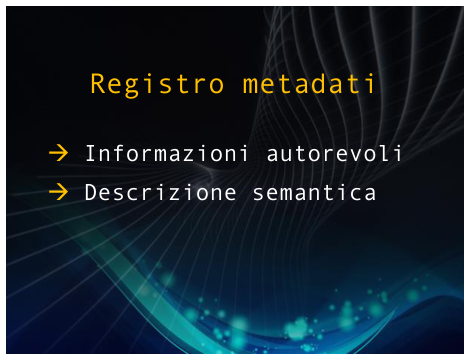
\includegraphics[width=0.50\textwidth,
                    trim=40 150 40 60, % L B R T
                    clip]
                    {images/Lez10_p04_fig_04}
  % \caption{Sommario}
  % \label{fig:Lez15_p06_fig_02}
\end{figure}
\FloatBarrier
\noindent

I metadata sono accompagnati da un registro che descrive quali sono le informazioni autorevoli, che indica che caratteristica devono avere le informazioni per poter essere considerate autorevoli e dà una descrizione semantica di questi dati, quindi una definizione del loro significato, attributi, eventuali relazioni tra piu lingue per l'uso in piu lingue di questi dati e anche relazioni tra diversi schemi di registri di metadata.

Alla fine di questo argomento vi propongo questo spunto.
Come gestite i contenuti nella vostra attività lavorativa o formativa o come sono gestiti dalla figura funzionale che è addetta a questa attività?

Inoltre quali sono gli strumenti tecnologici impiegati o che voi impiegate, quali attività sono supportate?

\section{Evoluzione storica dell'enterprise content management}

\FloatBarrier
\begin{figure}[H]
  \centering
  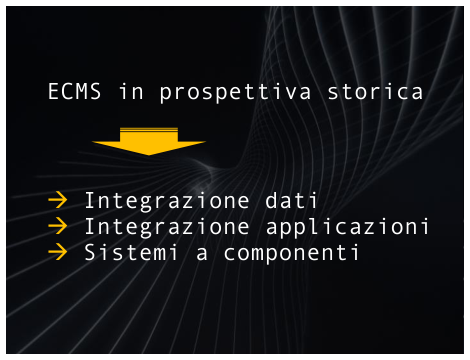
\includegraphics[width=0.50\textwidth,
                    trim=40 80 30 60, % L B R T
                    clip]
                    {images/Lez10_p05_fig_02}
  % \caption{Sommario}
  % \label{fig:Lez15_p06_fig_02}
\end{figure}
\FloatBarrier
\noindent

Considerando l'ECMS in una prospettiva storica, vediamo che possono essere individuate 3 fasi.

L'integrazione dei dati o ECMS sono stati orientati, costruiti, spinti soprattutto da necessità che provenivano dalla integrazione dei dati seguita dalla integrazione di applicazione, sistemi specifici per arrivare ai sistemi a componente, sistemi che partono da una base general purpose per essere estesi, specializzati a configurazioni aggiungendo delle componenti a mosaico.

\FloatBarrier
\begin{figure}[H]
  \centering
  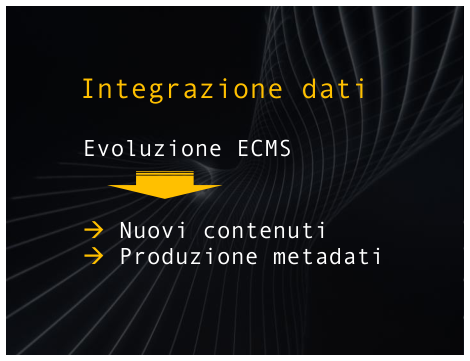
\includegraphics[width=0.50\textwidth,
                    trim=40 80 30 60, % L B R T
                    clip]
                    {images/Lez10_p05_fig_03}
  % \caption{Sommario}
  % \label{fig:Lez15_p06_fig_02}
\end{figure}
\FloatBarrier
\noindent

L'integrazione dei dati ha indotto una evoluzione dei CMS, dalla disponibilità di nuovi contenuti di vario genere, di tipo messaggio, quindi la necessità di gestire email piuttosto che messaggi di conversazioni estemporanee piuttosto che scambi avvenuti in social community, pagine, documenti e dalla produzione conseguente di metadata sia automatici, sia manuali, sia riguardanti il tempo d'uso dei vari documenti, la validità, i tempi di modifica, insomma i documenti, le informazioni che circolano per la rete sono diventati più complessi e hanno spinto le tecnologie di supporto al content management a evolvere verso l'elaborazione, l'organizzazione dei dati e verso la loro descrizione.

\FloatBarrier
\begin{figure}[H]
  \centering
  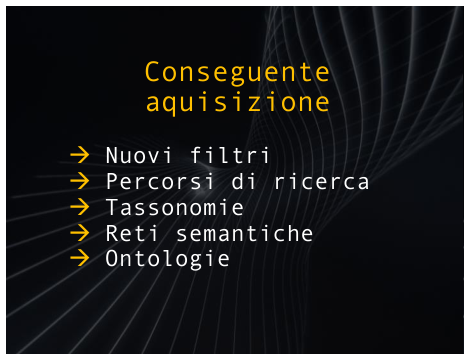
\includegraphics[width=0.50\textwidth,
                    trim=40 80 40 40, % L B R T
                    clip]
                    {images/Lez10_p05_fig_04}
  % \caption{Sommario}
  % \label{fig:Lez15_p06_fig_02}
\end{figure}
\FloatBarrier
\noindent

Conseguentemente sono stati acquisiti, sviluppati nuovi filtri per l'analisi per il recupero dei dati.
Lo sviluppo di percorsi per la ricerca o, visto dall'altra parte, organizzazioni delle informazioni differenti, sono state prodotte tassonomie per la loro organizzazione, classificazione o categorizzazione, reti semantiche, strutture più complesse e dedicate alla strutturazione piuttosto che alla produzione della struttura dei contenuti accompagnate anche da mappe mentali piuttosto che da altri tipi di rappresentazione del pensiero dei contenuti.

Per finire con le ontologie che sono rappresentazioni formalizzate dei concetti delle loro relazioni ed insiemi di regole per permettere ragionamenti formalizzati e eventualmente automatizzati a partire da questa base concettuale.

\FloatBarrier
\begin{figure}[H]
  \centering
  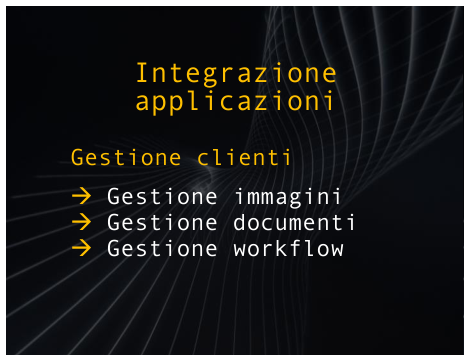
\includegraphics[width=0.50\textwidth,
                    trim=40 80 40 40, % L B R T
                    clip]
                    {images/Lez10_p05_fig_05}
  % \caption{Sommario}
  % \label{fig:Lez15_p06_fig_02}
\end{figure}
\FloatBarrier
\noindent

La fase successiva è quella dell'integrazione delle applicazioni.
Consideriamo per esemplificare un ambito in reparto di gestione dei clienti, farà uso di sistemi di gestione delle immagini per eventuali fotografie dei prodotti piuttosto che copie degli ordini, copie delle lettere, immagini da proporre ai clienti, immagini che riproducono qualche oggetto inviato dal cliente per un non funzionamento o per un altro tipo di documentazione.

La gestione di documenti a supporto contenuti trasportati proprio attraverso documenti o articoli piuttosto che pagine e eventualmente la gestione delle attività.

Qui per la gestione delle attività possiamo considerare che per esempio in un sistema di gestione delle relazioni con il cliente o anche solo in un sistema che ci permette l'automazione della gestione di un ordine, possono essere controllate le varie sottoattività, i vari task che devono essere svolti e controllati, mandato un messaggio per attivare l'attività, il task successivo per verificare l'effettuazione e la correttezza dello svolgimento di ogni attività.

\FloatBarrier
\begin{figure}[H]
  \centering
  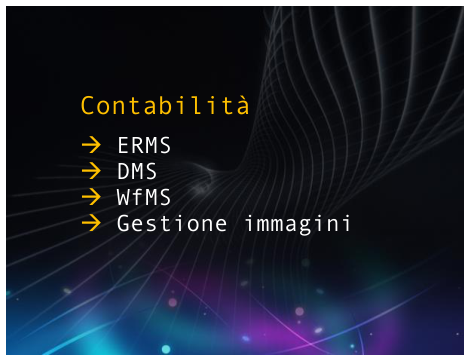
\includegraphics[width=0.50\textwidth,
                    trim=40 100 40 40, % L B R T
                    clip]
                    {images/Lez10_p05_fig_06}
  % \caption{Sommario}
  % \label{fig:Lez15_p06_fig_02}
\end{figure}
\FloatBarrier
\noindent

Un altro caso, per esempio un caso di contabilità, utilizzano sistemi ERMS, sistemi per l'enterprise resource management, piuttosto che sistemi di gestione dei documenti, document management system, per la documentazione eventualmente testuale da legare ai dati contabili; possono fare uso anche di workflow management system o ancora alla gestione di immagini.

Ecco che questo tipo di attività fanno uso di applicativi, di sistemi con finalità specifiche molto differenti e hanno richiesto quindi una forte integrazione di questi sistemi specifici.

\FloatBarrier
\begin{figure}[H]
  \centering
  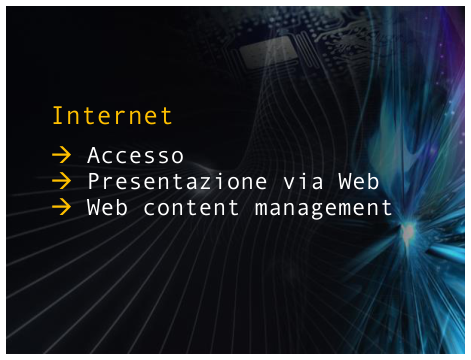
\includegraphics[width=0.50\textwidth,
                    trim=40 120 40 80, % L B R T
                    clip]
                    {images/Lez10_p06_fig_01}
  % \caption{Sommario}
  % \label{fig:Lez15_p06_fig_02}
\end{figure}
\FloatBarrier
\noindent


Inoltre internet ha aumentato la possibilità di accessi ad applicazioni differenti, di presentazione o richiede la presentazione anche attraverso questo nuovo canale e la gestione di web content, quindi la gestione di questi contenuti attraverso la rete con i nuovi protocolli e con i nuovi formati.

\FloatBarrier
\begin{figure}[H]
  \centering
  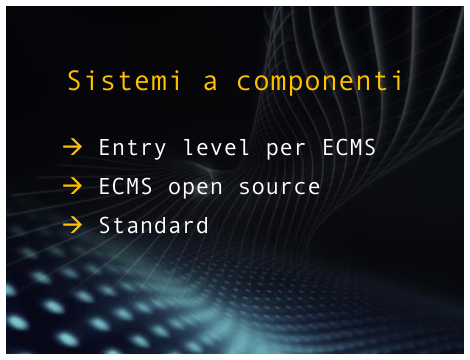
\includegraphics[width=0.50\textwidth,
                    trim=40 100 40 60, % L B R T
                    clip]
                    {images/Lez10_p06_fig_02}
  % \caption{Sommario}
  % \label{fig:Lez15_p06_fig_02}
\end{figure}
\FloatBarrier
\noindent

L'ultimo passo sono i sistemi a componenti.
Sono sono stati spinti nel 2006 quando Microsoft con la famiglia di prodotti SharePoint e Oracle con Oracle Content Management si sono uniti per definire un entry level quindi delle funzionalità di riferimento per gli ECMS.

Inoltre gli ECMS sono ora disponibili anche in versione open source come al fresco, logical doc, sense net e altri che permettono la modifica del sorgente quindi l'adattamento o l'estensione di nuove funzionalità da parte di tutta la comunità di utenti.

Stiamo parlando di versioni open source non necessariamente freeware quindi gratuite nella acquisizione.

Inoltre gli standard sono stati scatenanti e che includono gli standard come HIPAA, lo standard SAS 70 e altri.

Considero ora concluso questo argomento e vi propongo alcuni spunti di riflessione.

Usate un unico sistema software per la gestione dei contenuti o siete costretti per descrivere il content management system a cui dovete far riferimento nella vostra organizzazione a fare riferimento a più sistemi che utilizzate in maniera coordinata.

Il secondo punto è vorreste delle componenti aggiuntive e quali funzionalità vorreste che fossero aggiunte?
